\subsection{Spent Nuclear Fuel Simulations}
\label{sec:snfsim}

\begin{figure}[H]
  \centering
  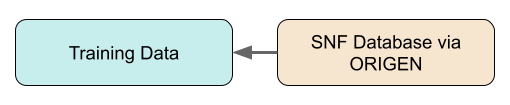
\includegraphics[width=0.7\linewidth]{./chapters/method/methodology1.png}
  \caption{First portion of the flowchart from Figure \ref{fig:method} being 
           described in this section.}
\end{figure}

Of interest to an entity trying to create a weapon is partially irradiated fuel
if they have plutonium separations capabilities or any radioactive substance in
the case of a dirty bomb. Thus, this work focuses on \gls{SNF} from commercial
power reactors. Ideally, a large enough database of \gls{SNF} nuclide assays
would be able to be used for this work. Since that does not exist, the 
database will be simulated via \gls{ORIGEN-ARP} \cite{origen, origenarp}.  

\subsubsection{Training Set Labels}
\label{sec:snflbls}

\begin{table}[!h]
  \centering
  \begin{subtable}{\linewidth}
    \centering
    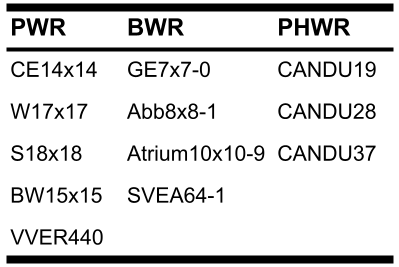
\includegraphics[width=0.5\linewidth]{./chapters/method/trainset4_Orxtrs.png}
    \caption{\gls{ORIGEN} designations for reactor technologies and fuel assembly design.}
    \label{tbl:rxtrtype}
    \vspace*{5mm}
  \end{subtable}
  \begin{subtable}{\linewidth}
    \centering
    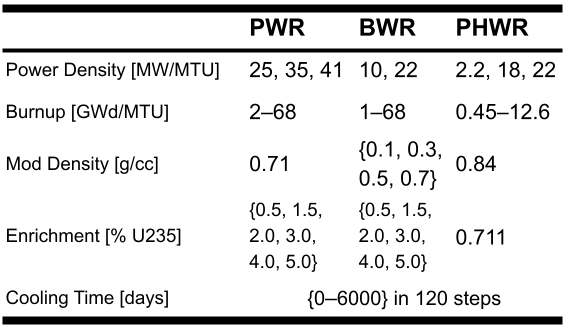
\includegraphics[width=0.75\linewidth]{./chapters/method/trainset4_inputs.png}
    \caption{Simulation parameters for \gls{ORIGEN} input files.}
    \label{tbl:rxtrparam}
  \end{subtable}%
  \caption{Training set database design using the \gls{SFCOMPO} database as guidance. \cite{sfcompo}}
  \label{tbl:train}
\end{table}

The design of the training set is dependent on a number of factors.  First, it
must have a sufficient number of burnup sets and time since irradiation steps
to provide robust prediction. This is decided upon by maximizing the steps for
both parameters, while balancing the computational limitations of a large
training set. Through previous experience, an approximate upper limit would be
somewhere around $1e6$ database entries for the specific calculations being
done in this work.

Secondly, the training set must represent what exists in the real world. This
was accomplished by studying the spread of parameters in the \gls{SFCOMPO}
database \cite{sfcompo}.  To ensure this, a variety of reactor types and
assembly designs were included, listed in Table \ref{tbl:rxtrtype}. Table
\ref{tbl:rxtrparam} lists the rest of the simulation inputs. These include not
only the labels of prediction interest, \gls{U235} enrichment, burnup, and time
since irradiation, but also other important simulation input parameters such as
the reactor power density and the moderator density.  (Water is both the
moderator and coolant in all simulated reactor types.)

\todo[inline]{add section reference} The third factor influencing database
design is ensuring ideal \gls{ML} algorithm performance.  As mentioned in
Section X, many algorithms are developed with the assumption that the training
set will be \acrfull{i.i.d.}.  This is important so that the model does not
overvalue or overfit a certain area in the training space. With the training
set design, there are predetermined values for enrichment, burnup, and time
since irradiation.  While there are $21-28$ burnup steps (depending on the
reactor type) and 120 cooling time steps, there are only 6 values for
enrichment. This creates the risk that the algorithm will end up being unable
to generalize outside of those discrete values. Therefore, the burnup steps and
time steps are perturbed randomly in a range that is $\pm10\%$ and $\pm30\%$
from the originally defined values, respectively.  The enrichment also gets
perturbed by $\pm10\%$, and not more because the cross-section libraries in
\gls{ORIGEN-ARP} are pre-calculated for those enrichment values, so deviating
too far from them would result in inaccurate \gls{SNF} simulations. The power
densities and moderator densities were kept at the values defined in Table
\ref{tbl:rxtrparam}.  The resulting training set is $5e5$.  Figure
\ref{fig:trainhist} visualizes the somewhat even distribution of the burnup and
cooling time parameters, and shows the lack of even distribution of the
enrichment parameter through a combination of scatter plots and histograms.
Note that there are many more \gls{BWR}s present in the histograms because of
the multiple moderator densities simulated (see Table \ref{tbl:rxtrparam})
\todo[inline]{update trainset size}

\begin{figure}[!htb]
  \makebox[\textwidth][c]{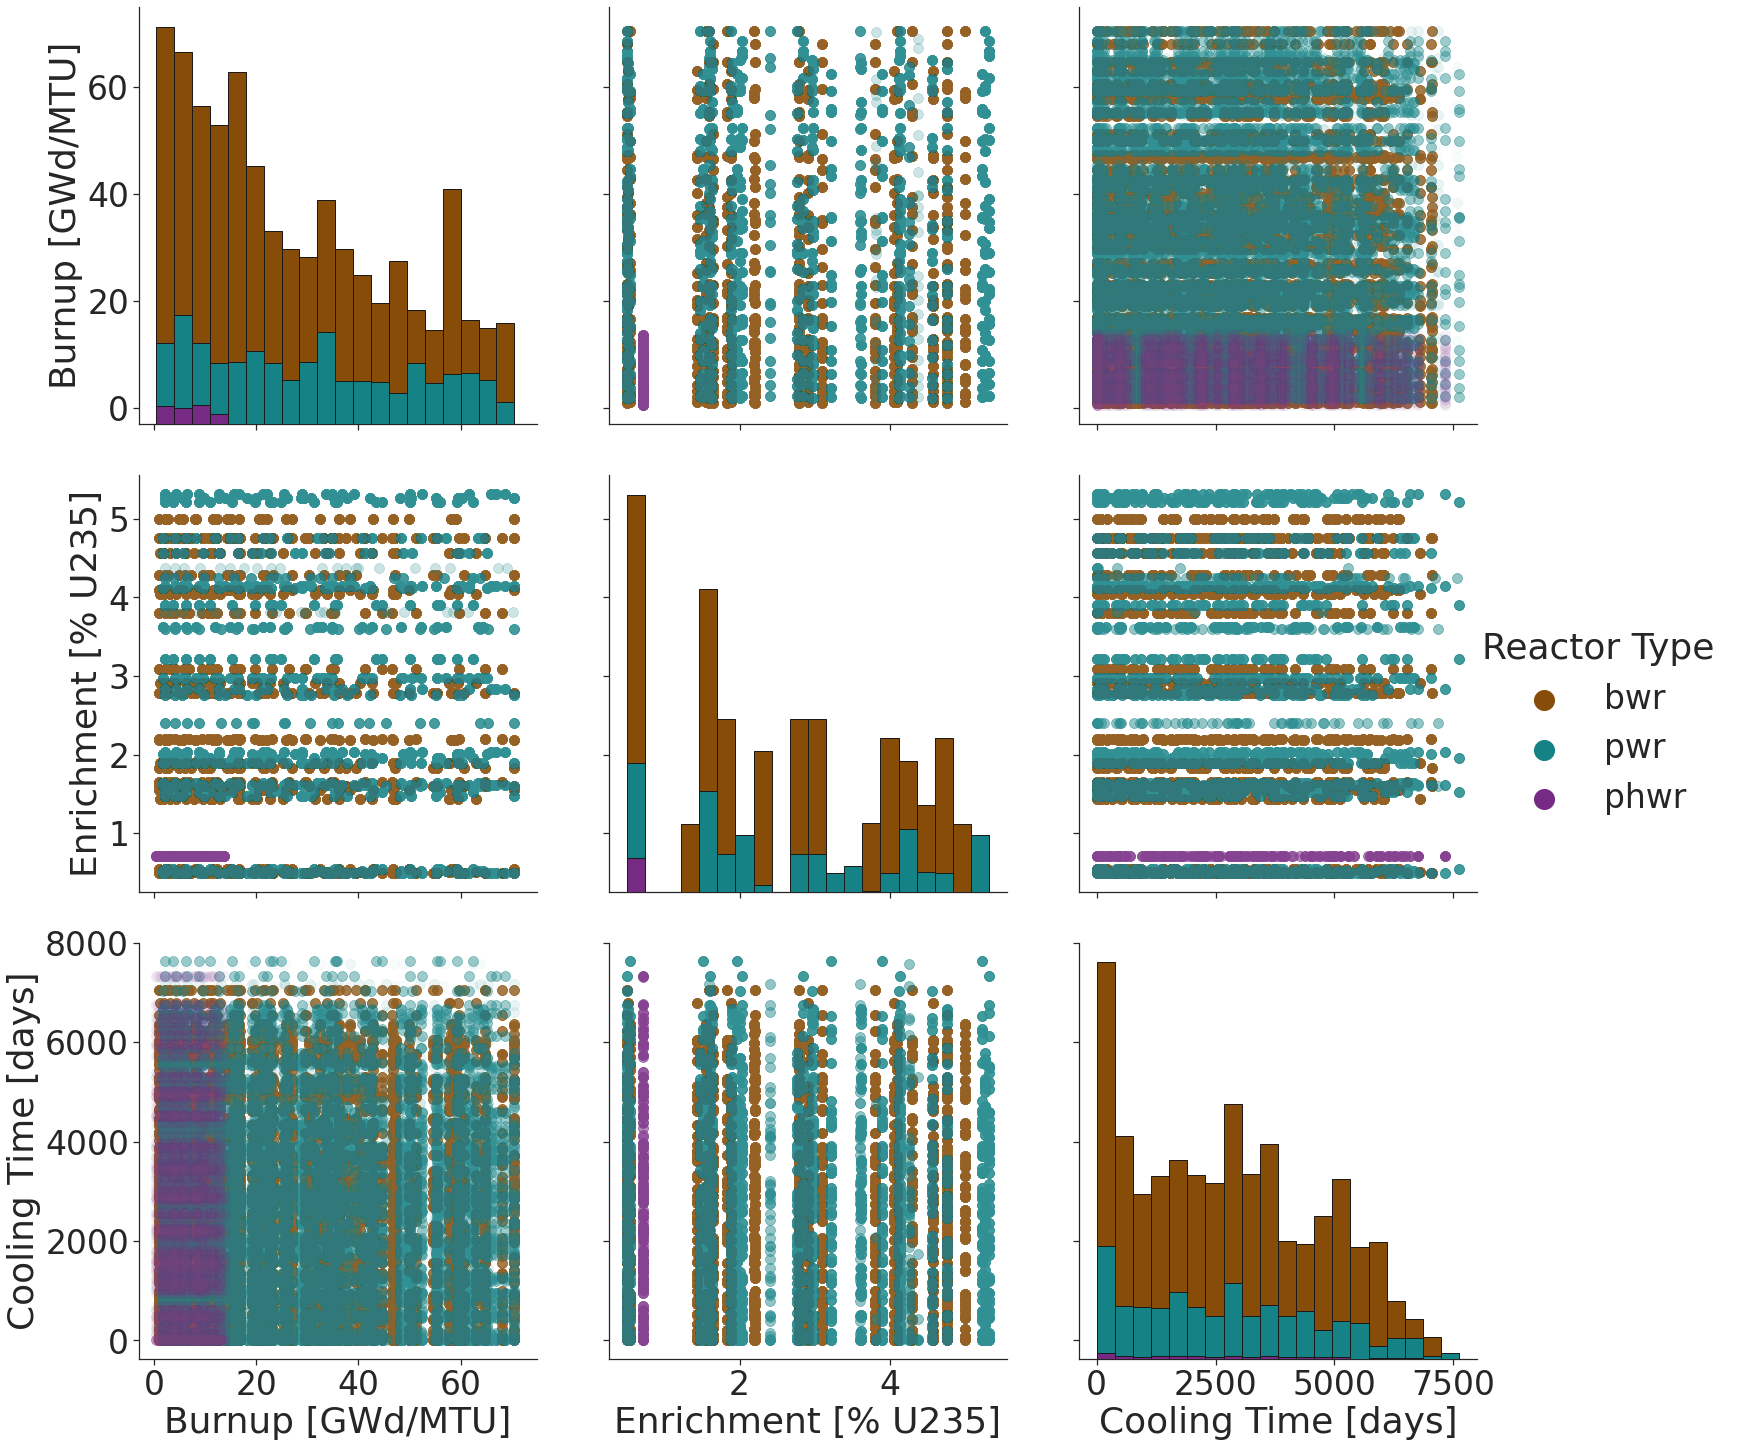
\includegraphics[width=\linewidth]{./chapters/method/histogram_scatter_trainset_viz.png}}
  \caption{A combination of histograms and scatter plots to visualize the 
           distribution of prediction labels in the training set.}
  \label{fig:trainhist}
  \todo[inline]{fix the histogram figure, this is a placeholder}
\end{figure}

\subsubsection{Training Set Features}
\label{sec:snffeats}

\todo[inline]{need to outline two exmpts before this. Writing this with that
assumption.} The other design decision regarding the training set is related to
which nuclides to track, i.e., the features.  For the first experiment, nuclide
masses are necessary, and the most common measurements in \gls{SFCOMPO} guide
the list of nuclides tracked.  In the second experiment, activities of
radionuclides are necessary to calculate gamma spectra from these values.

The first experiment with the 29 nuclide masses listed in Table
\ref{tbl:nucmass} was designed with the following reasons in mind.  First, the
units in mass is to represent the scenario of "perfect knowledge", where a full
assay is done via mass spectrometry techniques.  Second, this is to have the
training set units convertable to those present in the external, real-world
test set: the \gls{SFCOMPO} database.  The \gls{ORIGEN} simulations output the
nuclide masses in $grams$, and they are converted to the units of
\textit{milligrams per gram of initial uranium}, $mg/gU_i$, when the models are
externally tested against \gls{SFCOMPO}. Lastly, the 29 nuclides chosen were
based on the presence of measurements in \gls{SFCOMPO}, where these were
present in at least 100 of the samples in the database.  The test set is
described in more detail in Section \ref{sec:eval}.

\begin{table}[!h]
  \centering
  \begin{subtable}{\linewidth}
    \centering
    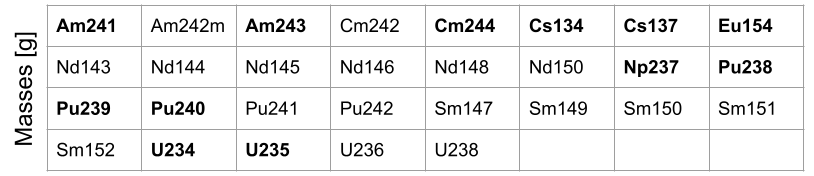
\includegraphics[width=\linewidth]{./chapters/method/nucmass_feats.png}
    \caption{Set of features saved for the first experiment, nuclide masses 
             measured in $grams$. The bold nuclide masses overlap with the 
             nuclides in \ref{tbl:nucacts}.}
    \label{tbl:nucmass}
    \vspace*{5mm}
  \end{subtable}
  \begin{subtable}{\linewidth}
    \centering
    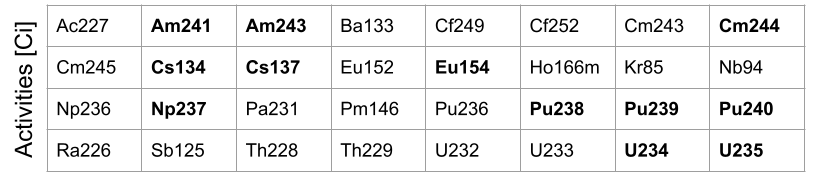
\includegraphics[width=\linewidth]{./chapters/method/nucacts_feats.png}
    \caption{Set of features saved for the second experiment, nuclide activities
             measured in $Curies$. The bold nuclide activities overlap with the 
             nuclides in \ref{tbl:nucmass}.}
    \label{tbl:nucacts}
  \end{subtable}%
  \caption{Two sets of features saved from the same simulation inputs for the 
           two main experiments in this work.}
  \label{tbl:nucfeats}
\end{table}

The second feature set with the 32 nuclide activities listed in Table
\ref{tbl:nucacts} was designed with the following reasons in mind. First,
nuclide activities are the most straightforward units to use for application to
the \gls{DRF} in the \gls{GADRAS} tool for the second experiment. This process
is used to obtain gamma spectra for each \gls{SNF} entry in the database, which
is detailed in \ref{sec:inforeduc}.  Second, these specific nuclides were
chosen because they fulfill four steps of filtering:
\begin{enumerate}
  \item They exist in the 196-long radionuclide list in \gls{GADRAS}.
  \item They have an activity above $1e-7\:Ci$ (cutoff chosen to filter out
  nuclides that are unlikely to produce gamma energy peaks).
  \item They have a half-life longer than $1\:year$ (cutoff chosen based on
  maximum cooling time of $16\:years$).
  \item They have at least one gamma energy line above $200\:keV$ (cutoff
  chosen based on low-energy gamma energy peaks being difficult to discern in
  some detectors).
\end{enumerate}

\subsubsection{Simulation Fidelity}
\label{sec:fidelity}

\todo[inline]{This section needs to be written about \gls{ORIGEN-ARP}
validation and maybe some nuclides that are known to perform poorly from ARP
sims. Can show a generic example from one of my sources, and or an example of
trying to match an \gls{ORIGEN-ARP} simulation to an \gls{SFCOMPO} entry.}

\subsection{Information Reduction}
\label{sec:inforeduc}

\begin{figure}[H]
  \centering
  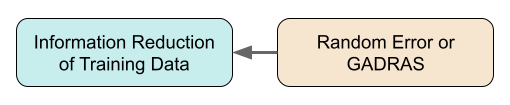
\includegraphics[width=0.7\linewidth]{./chapters/method/methodology2.png}
  \caption{Second portion of the flowchart from Figure \ref{fig:method} being 
           described in this section.}
\end{figure}

The overall goal of this project is to determine how much information to what
quality is needed to train an \gls{ML} model that can provide \gls{SNF}
attribution by correctly predicting the reactor type, burnup, \gls{U235}
enrichment, and time since irradiation.  In this section, the process of
information reduction of the training database is outlined for each experiment. 

The first experiment introduces the nuclide masses to a uniform uncertainty via
random error, and the second experiment computes a gamma spectrum for each
sample in the database from the nuclide activities in Section
\ref{sec:snffeats}.  This detector-based treatment is not being applied to the
mass measurements because studying measurement techniques that can only be done
in a lab is not the goal of this work.  Instead, field-deployable detectors are
of interest. \todo[inline]{make sure this is mentioned in the intro}

\subsubsection{1$^{\mathbf{st}}$ Experiment: Nuclide Masses}
\label{sec:masserr}

The training database for the first experiment is meant to be a proof of
principle with the developed methodology, and mimic a scenario where there is
"perfect knowledge" of a set of nuclides of interest. It is still interesting,
however, to probe how the statistical models perform under increasing error in
the nuclide measurements. Therefore error and uncertainty were injected into
the nuclide mass measurements in the training database for the machine learning
algorithms and \gls{MLL} calculations, respectively. 

\noindent \textbf{Machine Learning Algorithms} : For the \textit{k}-nearest
neighbor and decision tree algorithms, a uniform error is applied randomly to
each nuclide mass as follows.  For a maximum error $E_{max}$ between the values
of $0.0 < E_{max} < 0.2$, each nuclide mass is peturbed by a random fraction in
the range: $[1-E_{max},1+E_{max}]$.  Therefore the $0\%$ error case represents
full knowledge of nuclide masses, and that knowledge slowly decreases up to
$20\%$. 

\noindent \textbf{Maximum Likelihood Calculations} : For the \gls{MLL}
calculations, a uniform uncertainty was introduced to each nuclide mass.  Thus,
each nuclide is given an uncertainty of $5\%$, $10\%$, $15\%$, and $20\%$
via:
\begin{equation}
  \label{eq:mllunc}
  \sigma_{Log L}^2 = \sum_j \left( 
                            \frac{r_{j,test} - r_{j,sim}}{\sigma_{j,sim}^2}
                            \right)^2 
                            (\sigma_{j,sim}^2 + \sigma_{j,test}^2)
\end{equation}
where $r_{j,sim}$ and $r_{j,test}$ are the nuclide measurements for the
simulated/training set samples and the test samples, respectively, and
$\sigma_{j,sim}$ and $\sigma_{j,test}$ are their respective standard
deviations calculated from the four uncertainty levels listed above.

\subsubsection{2$^{\mathbf{nd}}$ Experiment: Gamma Spectra}
\label{sec:gamerr}

Moving beyond injecting uniform error to a nuclide mass measurement, the next
step in information reduction takes place for the second experiment, which uses 
processed gamma spectra for the training database. This adds more than one layer of 
reduced information quality, which are listed here as an outline of the steps
taken to process the gamma spectra:
\begin{enumerate}
  \item \label{itm:1} The list of nuclides is limited to radionuclides.
  \item \label{itm:2} Instead of "perfect" radionuclide activity knowledge, 
        they are being measured by a gamma detector.
  \item \label{itm:3} The processing of the gamma spectra can be highly variable.
  \item \label{itm:4} The $\sqrt{n}$ error of counts-based detection is included. 
\end{enumerate}

Step \ref{itm:1} covers which radionuclides to include, which was previously
covered in Section \ref{sec:snffeats}. Step \ref{itm:2} is to obtain a gamma
spectrum for every \gls{SNF} entry in the database. This is done using the
\gls{GADRAS} tool, which applies a \gls{DRF} to the gamma lines from these
radionuclides. The input is a nuclide activity vector, and the output is an
array of energy bins (measured in $keV$), and the counts per energy bin.

The nuclide activity data did require some processing to be used in this way.
The activities that come from the \gls{ORIGEN} simulations are based on there
being $1\:MT$ of initial uranium-based fuel. Not only is this quantity an
unlikely amount to be smuggled, it would overwhelm a detector at the
\todo[inline]{fix this to be better technical explanation of dead time and pile
up} source-detector distances in \gls{GADRAS}. Therefore, the material (and
resulting nuclide activities) are scaled to be $1\:g$ of \gls{SNF}.

Regarding the input information for the \gls{GADRAS} calculations, the sources
are provided without any background; this is because any spectrum would undergo
background subtraction before further analysis. Additionally, the nuclides are
pre-decayed in \gls{ORIGEN} to correspond to various cooling times, but the
source age provided to \gls{GADRAS} needs to be a non-zero value. A source age
of $20\:minutes$ provides the expected peaks.

\begin{table}[!h]
  \centering
  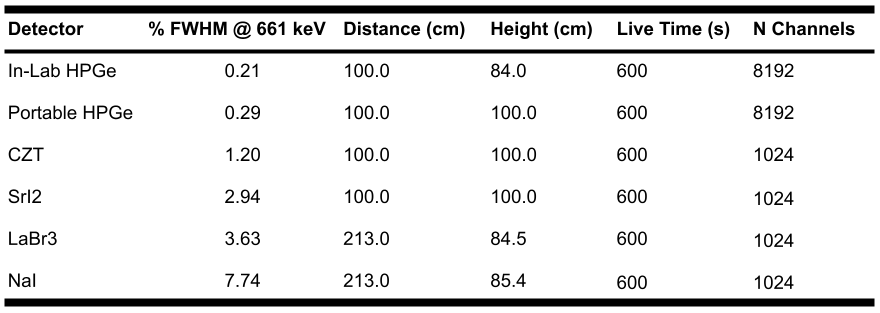
\includegraphics[width=\linewidth]{./chapters/method/gadras_detectors.png}
  \caption{Select details of 6 detector setups used to obtain gamma 
           spectra-based training databases.}
  \label{tbl:detsetups}
\todo[inline]{update this table if live times for nai and labr3 change}
\end{table}

Training databases were created for the six detectors outlined in Table
\ref{tbl:detsetups}. They were chosen to compare the highest energy resolution
detector, a lab-based \gls{HPGe}, against the rest, in order of decreasing
energy resolution: portable \gls{HPGe}, \gls{CZT}, \gls{SrI2}, \gls{LaBr3}, and
\gls{NaI} detectors. This is displayed in the table by including the \gls{FWHM}
of the $661\:keV$ peak for Cs137. At this point, there are six versions of the
original database for each detector setup, but there is a full gamma spectrum
for each \gls{SNF} entry. It is not computationally prudent to use full gamma
spectra for training and testing, and so these spectra are processed; this is
step \ref{itm:3} from above, and is outlined as follows.

\begin{figure}[!h]
  \makebox[\textwidth][c]{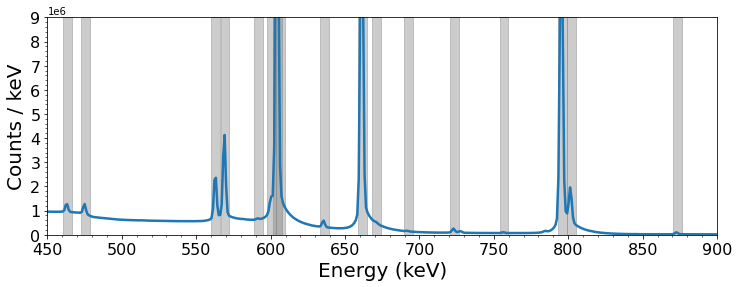
\includegraphics[width=\linewidth]{./chapters/method/energy_window_example.png}}
  \caption{Slice of an example gamma spectrum in one of the training databases
           showing the windows over the gamma energy peaks.}
  \todo[inline]{update}
  \label{fig:enwindows}
\end{figure}



\begin{table}[!h]
  \centering
  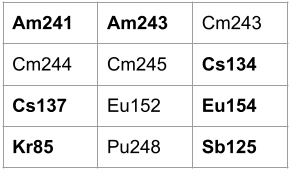
\includegraphics[width=0.4\linewidth]{./chapters/method/enlist_nucs.png}
  \caption{Nuclides that are represented by the gamma energy lines in the two . The entire 
           set of 11 nuclides belongs to the long list, and the 6 bold nuclides
           belong to the short list.}
  \label{tbl:enlistnucs}
\todo[inline]{this is for edited energy window lists, and includes problematic (simulation-wise) nuclides.}
\end{table}

Lastly, step \ref{itm:4} involves the inclusion of the counting error for the
summed energy windows. This is quite simple, as statistical counting error of
$n$ counts is $\sqrt{n}$.  As in Section \ref{sec:masserr}, this error gets
applied in the same way for the machine learning algorithms, where the uniform
error is applied randomly within the range $[r-\sqrt{r},r+\sqrt{r}]$ for each
summed energy window $r$. For the \gls{MLL} calculations, Equation
\ref{eq:mllunc} is used, where $\sigma_{j} = \sqrt{r}$.  \todo[inline]{make
sure variables are explained clearly, choosing r to match variables above, the
original variable choice comes from TAMU papers}
